\documentclass{article}

\usepackage[margin=1in,includefoot]{geometry}

%graphics preamble
\usepackage{graphicx} %allow import images
\usepackage{float} %allow control of float position

\begin{document}

\begin{titlepage}
	\begin{center}
		\line(1,0){300}\\
		[0.25in]
		\huge{\bfseries Monopoly assistance}\\
		[2mm]
		\line(1,0){200}\\
		[1.5cm]
		\textsc{\LARGE ElHadi73}\\
		[0.75cm]
		\textsc{\Large Development report and documentation}\\
		[10cm]
	\end{center}
	\begin{flushright}
		\textsc{\large ElHadi73\\
		Mars 28, 2023\\}
	\end{flushright}
\end{titlepage}

%the page numbering before table of content is in roman
\pagenumbering{roman}

%this is the table of content page
\cleardoublepage
\tableofcontents
\thispagestyle{empty}
\cleardoublepage

%the page numbering after table of content is in arabic
\pagenumbering{arabic}

%restart counting pages from 1
\setcounter{page}{1}

\section{Introduction}\label{sec:intro}
        The classic board game Monopoly has been enjoyed by millions of people of all ages for over eight decades. It is a game that involves buying, selling, and trading properties with the objective of becoming the wealthiest
player. Monopoly has brought joy to countless families and friends over the years. However, the game's reliance on paper money and too many physical game pieces can make it cumbersome and time-consuming to play.

        Monopoly Assistantante is a digital app designed to enhance and simplify the gameplay experience of the classic board game Monopoly for an efficient and convenient way to play the game by providing a digital system for managing players money and properties, reducing the amount of paper used during gameplay, and tracking game progress in real-time, and make it less time-consuming, with customizable rules featuer with multiplayer support, and try to achive that without sacrificing the social and fun aspects of playing in person. 

        These features aim to simplify the gameplay experience for players while also enhancing it by providing real-time updates, detailed statistics, and customizable options. 
        In addition, the app's digital tracking capabilities allow players to easily view their progress throughout the game, including their assets, properties, and overall net worth. This provides players with a clear understanding of their current position and helps them make more informed gameplay decisions. By providing players with a comprehensive overview of the game, Monopoly Assistantante can also help players develop their strategic thinking and decision-making skill, which can lead to a more immersive and engaging experience, where players can fully explore the strategic depth of the game and gain valuable experience in theory.  

	The thesis will evaluate the effectiveness of the app in improving the Monopoly gameplay experience, with a focus on how it impacts gameplay mechanics, and the flow and speed of the game, facilitates more strategic gameplay, player interaction, and overall enjoyment, as well as to identify areas for potential future development.

        It is important to note that while the app is designed to reduce the amount of paper used and make gameplay more efficient, it is not intended to replace the physical presence of the players and the board game itself. The fun and social aspects of playing Monopoly in person are an essential part of the game's appeal, and the app is designed to complement and enhance these aspects, rather than replace them.

        The thesis will begin by reviewing the literature on board games and digital technology, as well as discussing the design and development process of the app. Next, the thesis will present the results of user testing and surveys to evaluate the app's usability and user experience. Finally, the thesis will conclude with a discussion of the findings and potential directions for future research in this area.
        Through an analysis of Monopoly Assistantante's features and impact on gameplay, this thesis aims to explore the ways in which digital tools can enhance and modernize traditional board game experiences. By examining the app's impact on gameplay mechanics, player interaction, and enjoyment, this thesis seeks to provide valuable insights into the role of technology in transforming classic board games into efficient and engaging digital experiences.

\section{Problematic}\label{sec:prbm}
Playing monopoly is really fun, but it take a lot of time, which causes many of your friends refuses to play it, that what will make playing it not fun.
one of the things that causes it to take very long is the money transactions between players, or with the bank/goverment, espacaly when u dont have the change to pay the right amount of money.

\section{Objectives}\label{sec:obj}
in this web app we will minimize the time it takes to make a transaction between two players or between a player and the bank/goverment, where the transactions going to be made digitly, and the money holding will be virtually.

\section {System Requirements and Actors}
\subsection {Introduction}
To make sure that the web application replaces the paper money its full uses in the game, it is important to identify the diffrent user of the system

\subsection {User Actors}
	\subsubsection {Admin}
 An external user who is an administrator of the system and can access a set of use cases related to managing the game
	\subsubsection {Guest}
An external user who is not a registered player or administrator and can access a limited set of use cases
	\subsubsection {Player}
 An external user who is a registered player and can access a set of use cases related to playing the game
\subsection{Static Context Diagram}
 \begin{figure}[H]
	 \centering
	 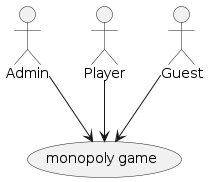
\includegraphics[height=3in]{../thesis_tex/assets/diagrams/SCD.png}
	 \caption{Static Context Diagram}
\end{figure}

\subsection{Functional Requirements}
\subsubsection{Global}
-The system will be capable of handling all money transactions between all element of the game according to the game rules
-Each game will have an administrator
-A player or Admin must go through guest fase
\subsubsection{Guest}
-Guest Can choose between hosting a new game or joining an already started game
\subsubsection{Admin}
-Can initiate transactions of money between players and the Bank
\subsubsection{Player}
-Can initiate money transaction to other entities of the game

\subsection{Non-Functional Requirements}
\subsubsection{Game rules}
-All transaction must be logged as histroy of transacion
-The histroy of transacion must be available of all players to see
-Any money transaction must be accepted or refused by admin of the game before it is made
-In futur Version all game rules can be customizable by Admin of the game
-All transaction must be valudated first by admin
-The admin is not the same person, but in futur version the admin can switch between player and admin roles
-All user must loggin to use the system
-The UI/UX must be responsive
\subsubsection{Security}
-Authentication and authorization: The website must have a robust authentication and authorization mechansime in place to ensure that only authorized users can access there data or perform critical actions that they are allowed to do.
-Protection against SqlInjections Attack
\subsubsection{Usability}
\subsubsection{Performance}
\subsubsection{Relability}
\subsubsection{Scalability}
\subsubsection{Maintainability}
\subsubsection{Compatibility}

\subsection{Conclusion}

\section {understanding the monopoly game}
\subsection { the money flow in monopoly }
 \begin{figure}[H]
	 \centering
	 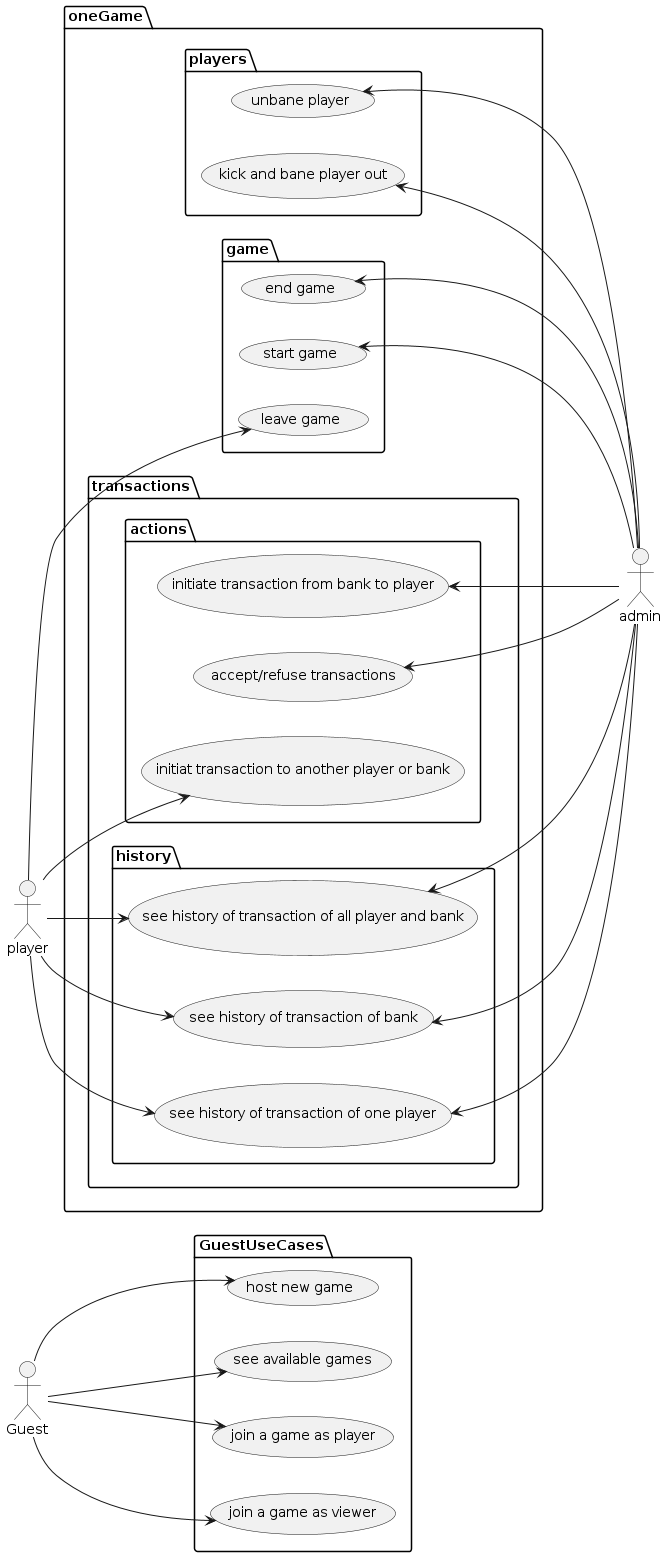
\includegraphics[height=7in]{../thesis_tex/assets/diagrams/global_ucd.png}
	 \caption{Global Usecase Diagram}
\end{figure}

\section{Architecture and Design}

\subsection{Introduction}

\cleardoublepage
\subsection{Global Usecase Diagram}
 \begin{figure}[H]
	 \centering
	 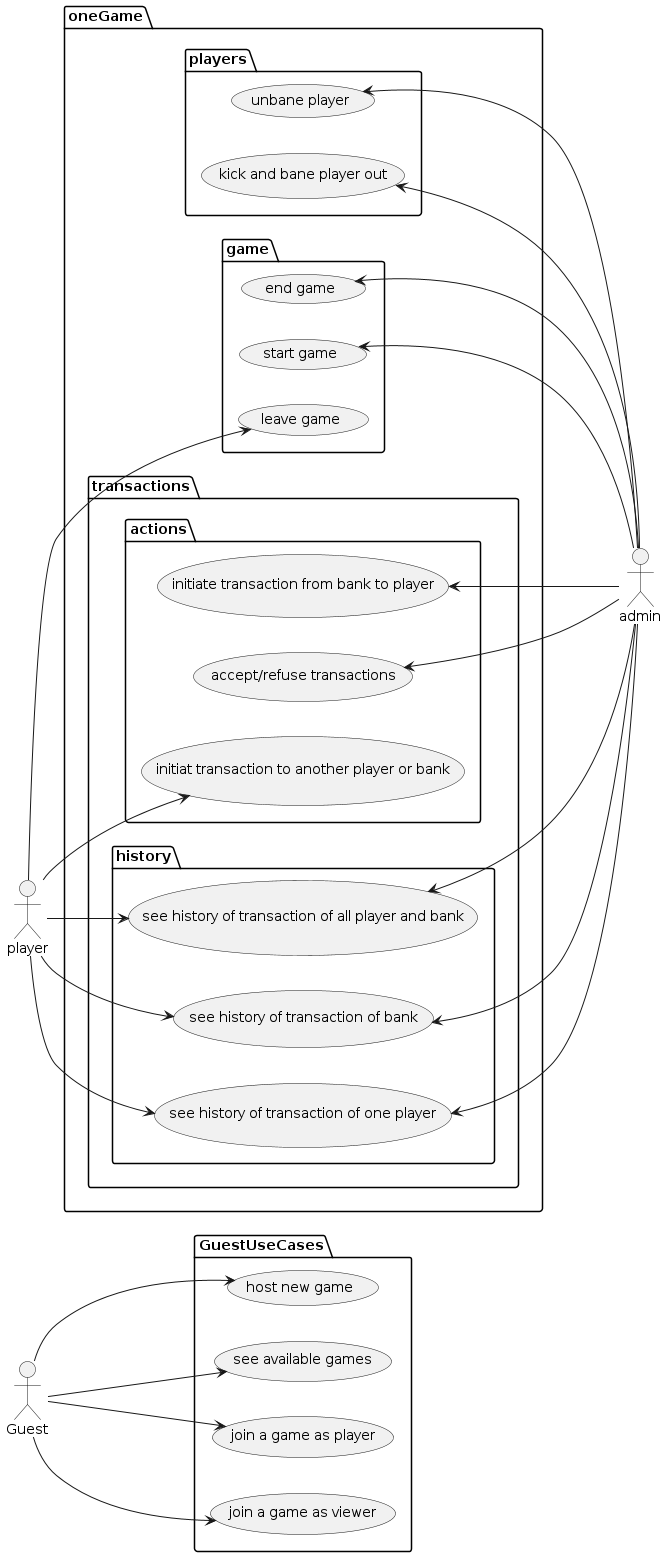
\includegraphics[height=7in]{../thesis_tex/assets/diagrams/global_ucd.png}
	 \caption{Global Usecase Diagram}
\end{figure}
\cleardoublepage

\subsubsection{Guest Usecase Diagram}
 \begin{figure}[H]
	 \centering
	 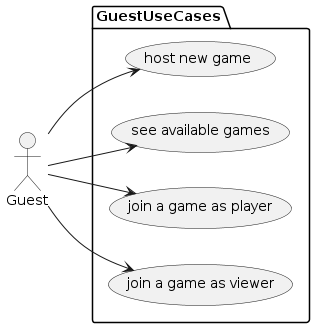
\includegraphics[height=3in]{../thesis_tex/assets/diagrams/guest_ucd.png}
	 \caption{Guest Usecase Diagram}
\end{figure}

\cleardoublepage
\subsubsection{Admin Usecase Diagram}
 \begin{figure}[H]
	 \centering
	 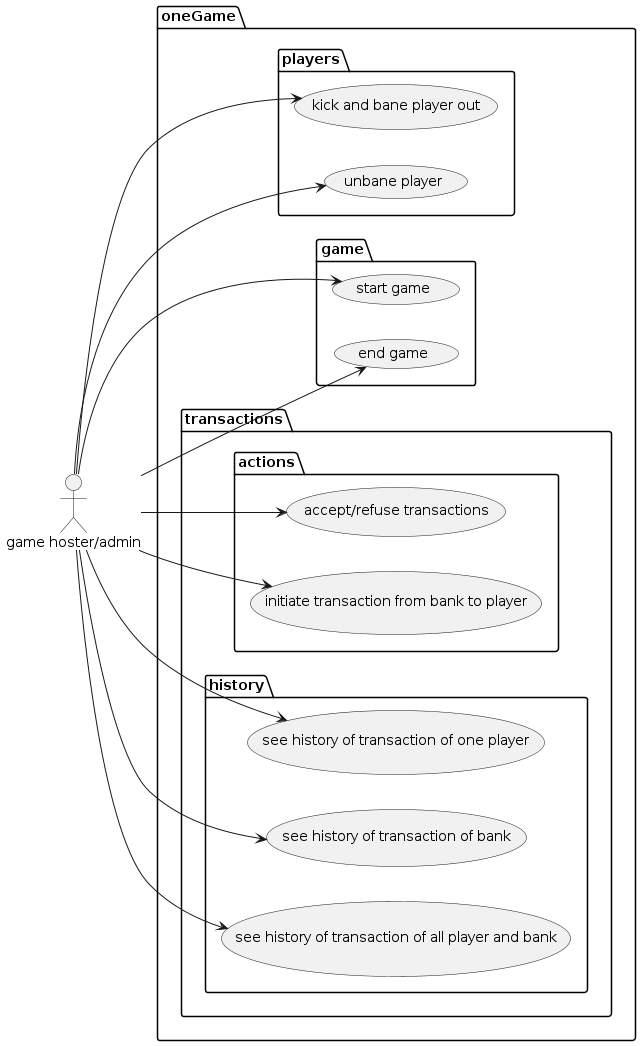
\includegraphics[height=7in]{../thesis_tex/assets/diagrams/admin_ucd.png}
	 \caption{Admin Usecase Diagram}
\end{figure}
\cleardoublepage

\cleardoublepage
\subsubsection{Player Usecase Diagram}
 \begin{figure}[H]
	 \centering
	 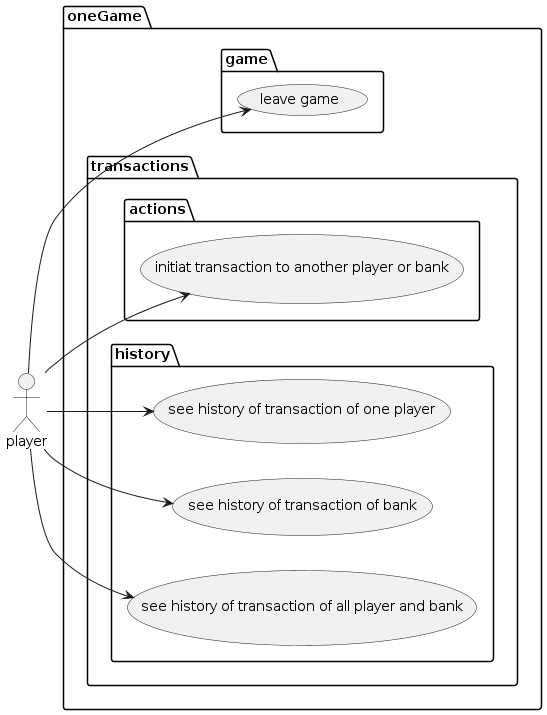
\includegraphics[height=7in]{../thesis_tex/assets/diagrams/player_ucd.png}
	 \caption{Player Usecase Diagram}
\end{figure}
\cleardoublepage

\subsection{Usecases Study}
\subsubsection{Host new game by the guest actor usecase}
 \begin{figure}[H]
	 \centering
	 \includegraphics[height=3in]{../thesis_tex/assets/diagrams/guest_host_game_SD.png}
	 \caption{Host new game by the guest actor Sequence Diagram}
\end{figure}

 \begin{figure}[H]
	 \centering
	 \includegraphics[height=3in]{../thesis_tex/assets/diagrams/guest_host_game_detailedSD.png}
	 \caption{Host new game by the guest actor detailed Sequence Diagram}
\end{figure}

\subsubsection{show available games by the guest actor usecase}
 \begin{figure}[H]
	 \centering
	 \includegraphics[height=3in]{../thesis_tex/assets/diagrams/guest_show_available_games_SD.png}
	 \caption{Show available games by the guest actor Sequence Diagram}
\end{figure}

 \begin{figure}[H]
	 \centering
	 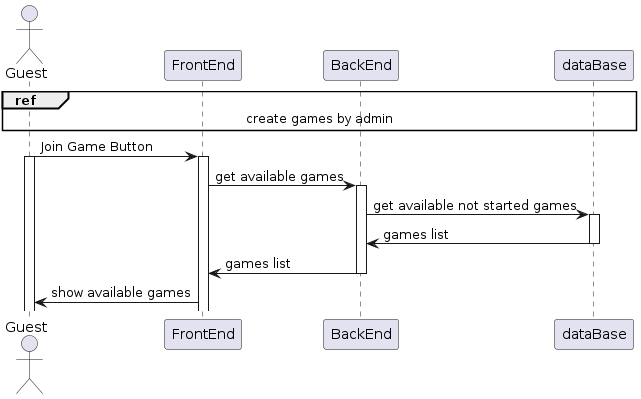
\includegraphics[height=3in]{../thesis_tex/assets/diagrams/guest_show_available_games_detailedSD.png}
	 \caption{Show available games by the guest actor detailed Sequence Diagram}
\end{figure}

\subsubsection{join game by the guest actor usecase}
 \begin{figure}[H]
	 \centering
	 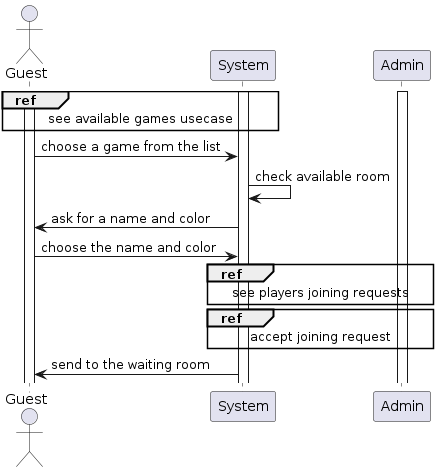
\includegraphics[height=3in]{../thesis_tex/assets/diagrams/guest_join_game_SD.png}
	 \caption{Join game by the guest actor Sequence Diagram}
\end{figure}

 \begin{figure}[H]
	 \centering
	 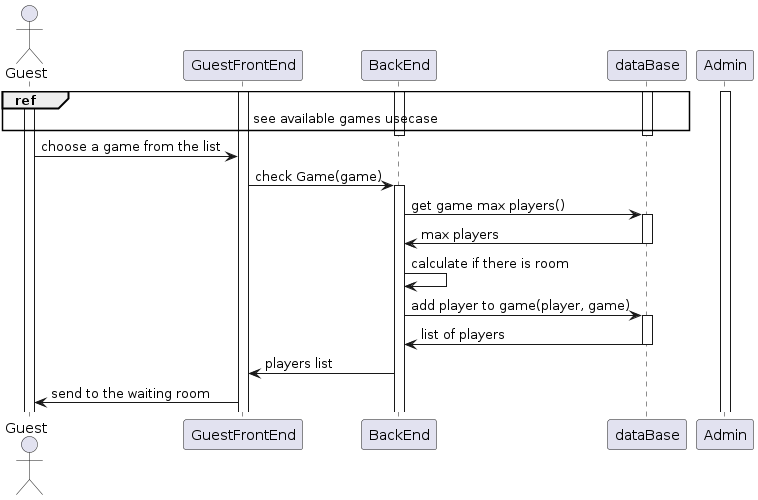
\includegraphics[height=3in]{../thesis_tex/assets/diagrams/guest_join_game_detailedSD.png}
	 \caption{Join game by the guest actor detailed Sequence Diagram}
\end{figure}

\subsubsection{start game by the admin actor usecase}
 \begin{figure}[H]
	 \centering
	 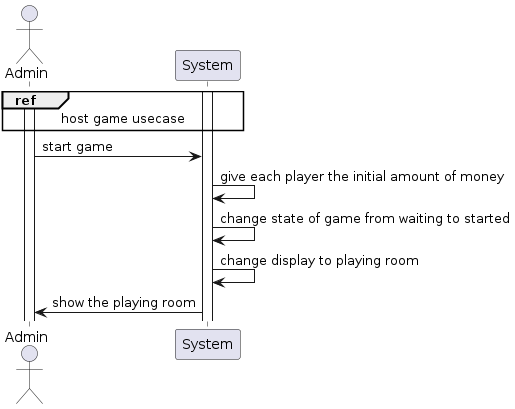
\includegraphics[height=3in]{../thesis_tex/assets/diagrams/admin_start_game_SD.png}
	 \caption{Start game by the admin actor Sequence Diagram}
\end{figure}

 \begin{figure}[H]
	 \centering
	 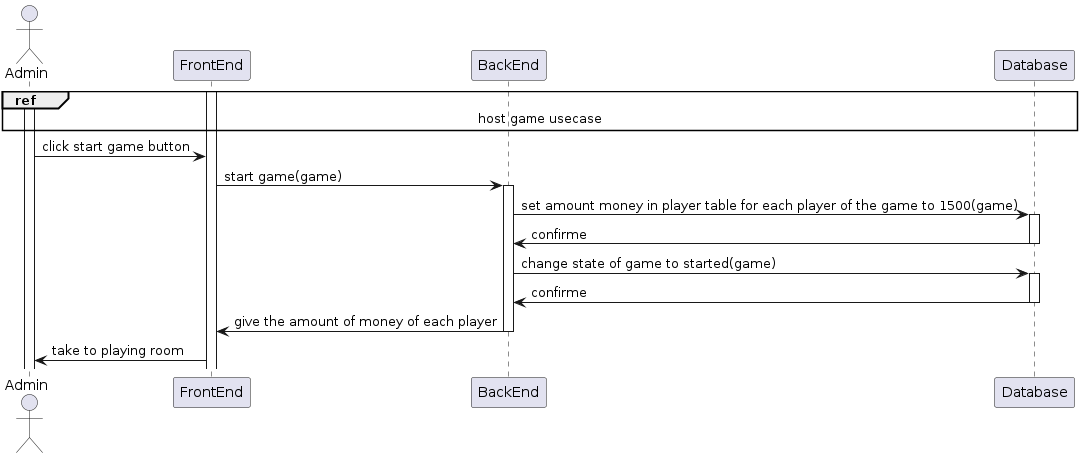
\includegraphics[height=3in]{../thesis_tex/assets/diagrams/admin_start_game_detailedSD.png}
	 \caption{Start game by the admin actor detailed Sequence Diagram}
\end{figure}

\subsubsection{kick player out by the admin actor usecase}
 \begin{figure}[H]
	 \centering
	 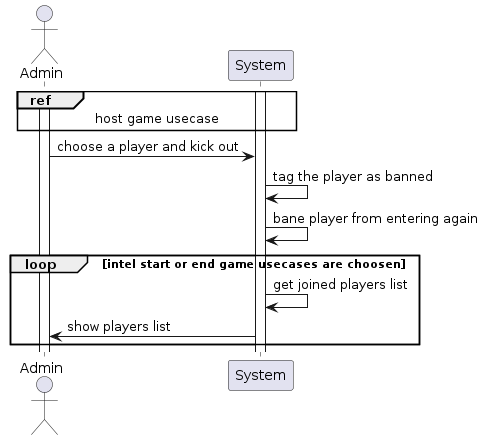
\includegraphics[height=3in]{../thesis_tex/assets/diagrams/kick_player_out_SD.png}
	 \caption{kick player out by the admin actor Sequence Diagram}
\end{figure}

 \begin{figure}[H]
	 \centering
	 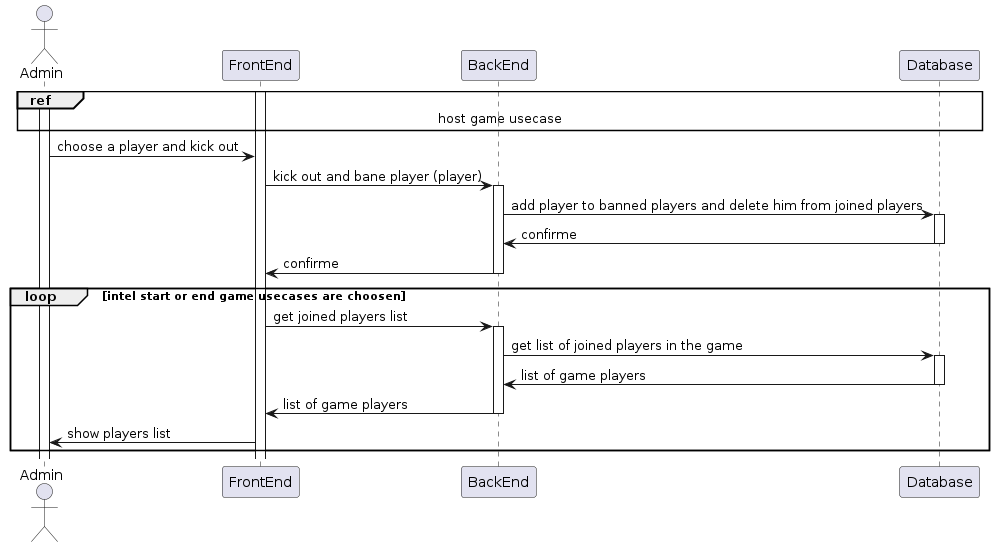
\includegraphics[height=3in,width=6in]{../thesis_tex/assets/diagrams/kick_player_out_detailedSD.png}
	 \caption{kick player out by the admin actor detailed Sequence Diagram}
\end{figure}

\subsubsection{unbane player by the admin actor usecase}
 \begin{figure}[H]
	 \centering
	 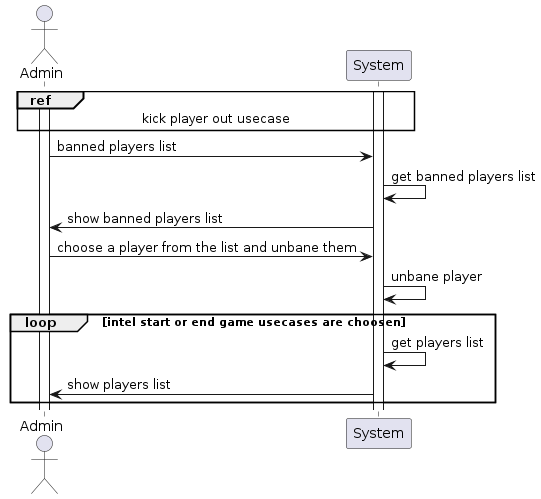
\includegraphics[height=3in]{../thesis_tex/assets/diagrams/unbane_player_SD.png}
	 \caption{unbane player by the admin actor Sequence Diagram}
\end{figure}

 \begin{figure}[H]
	 \centering
	 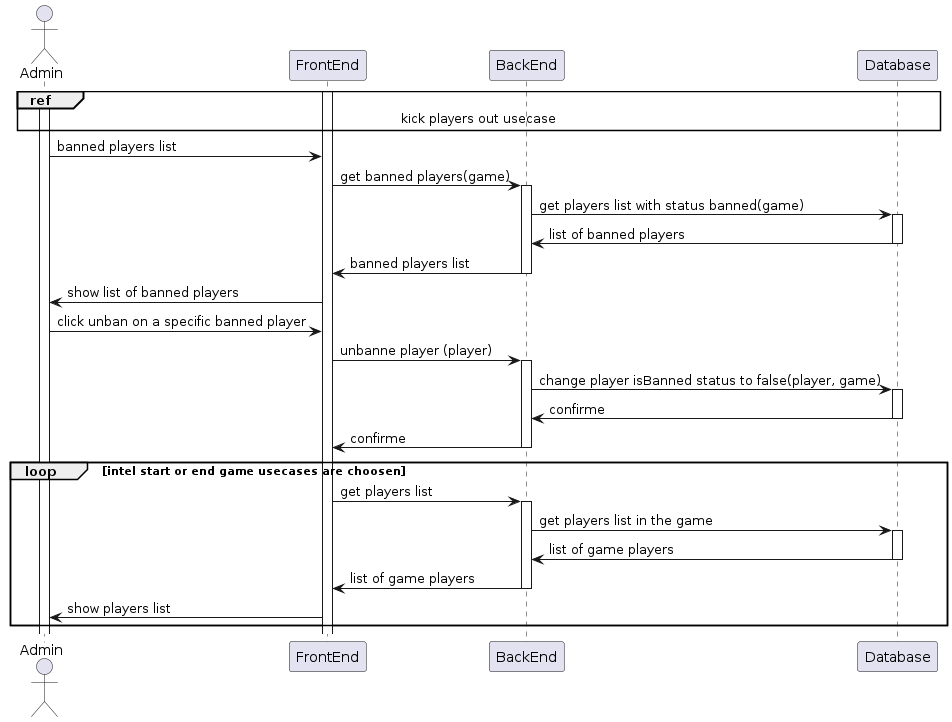
\includegraphics[height=4in,width=6in]{../thesis_tex/assets/diagrams/unbane_player_detailedSD.png}
	 \caption{unbane player by the admin actor detailed Sequence Diagram}
\end{figure}

\subsubsection{end game by the admin actor usecase}
 \begin{figure}[H]
	 \centering
	 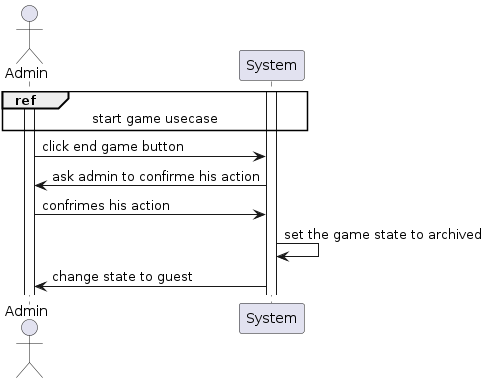
\includegraphics[height=3in]{../thesis_tex/assets/diagrams/admin_end_game_SD.png}
	 \caption{end game by the admin actor Sequence Diagram}
\end{figure}

 \begin{figure}[H]
	 \centering
	 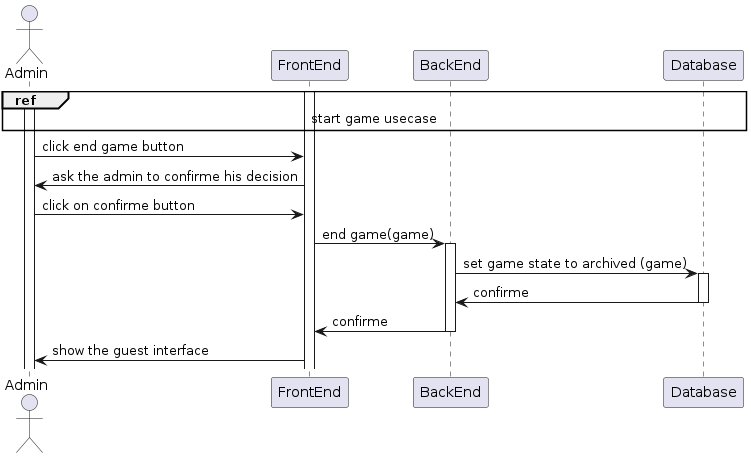
\includegraphics[height=3in]{../thesis_tex/assets/diagrams/admin_end_game_detailedSD.png}
	 \caption{end game by the admin actor detailed Sequence Diagram}
\end{figure}

\subsubsection{accept or refuse transaction by the admin actor usecase}
 \begin{figure}[H]
	 \centering
	 \includegraphics[height=3in]{../thesis_tex/assets/diagrams/accept_refuse_transaction_SD.png}
	 \caption{accept or rufuse transaction by the admin actor Sequence Diagram}
\end{figure}

 \begin{figure}[H]
	 \centering
	 \includegraphics[height=4in,width=6in]{../thesis_tex/assets/diagrams/accept_refuse_transaction_detailedSD.png}
	 \caption{accept or rufuse transaction by the admin actor detailed Sequence Diagram}
\end{figure}

\subsubsection{initiate transaction from the bank to another player by the admin actor usecase}
 \begin{figure}[H]
	 \centering
	 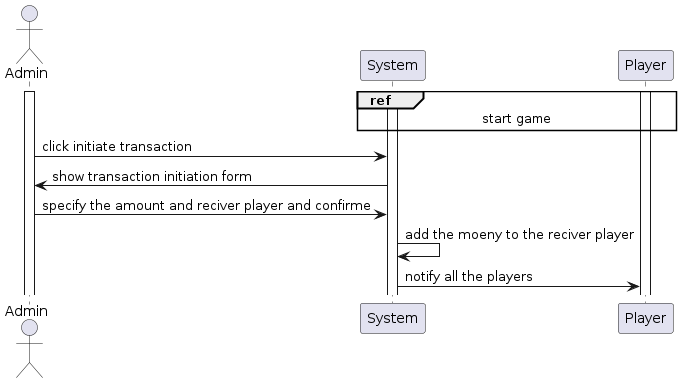
\includegraphics[height=3in]{../thesis_tex/assets/diagrams/initiate_transaction_to_another_player_SD.png}
	 \caption{initiate transaction from the bank to another player by the admin actor Sequence Diagram}
\end{figure}

 \begin{figure}[H]
	 \centering
	 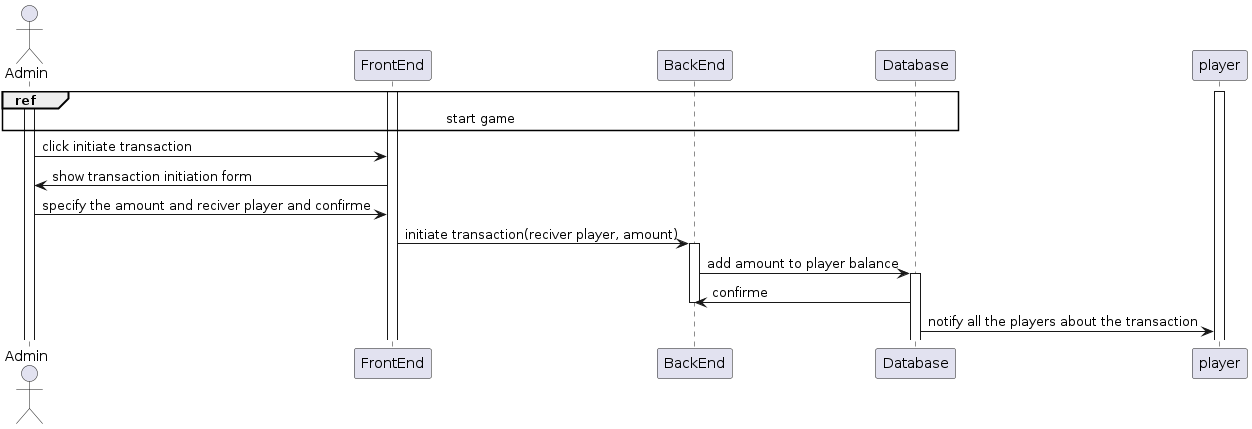
\includegraphics[height=3in,width=6in]{../thesis_tex/assets/diagrams/initiate_transaction_to_another_player_detailedSD.png}
	 \caption{initiate transaction from the bank to another player by the admin actor detailed Sequence Diagram}
\end{figure}

\subsubsection{see transactions full histroy by the admin actor usecase}
 \begin{figure}[H]
	 \centering
	 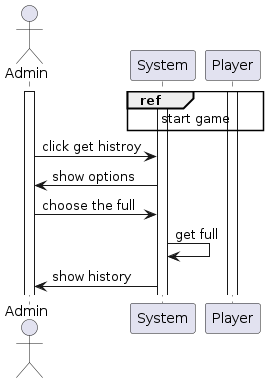
\includegraphics[height=3in]{../thesis_tex/assets/diagrams/see_transactions_full_history_SD.png}
	 \caption{see transactions full histroy by the admin actor Sequence Diagram}
\end{figure}

 \begin{figure}[H]
	 \centering
	 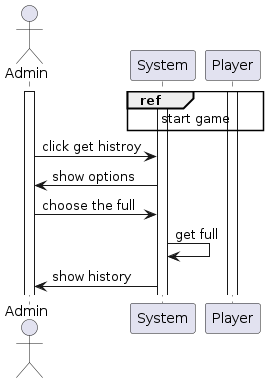
\includegraphics[height=4in,width=6in]{../thesis_tex/assets/diagrams/see_transactions_full_history_detailedSD.png}
	 \caption{see transactions full histroy by the admin actor detailed Sequence Diagram}
\end{figure}

\subsubsection{see transaction histroy of the bank by the admin actor usecase}
 \begin{figure}[H]
	 \centering
	 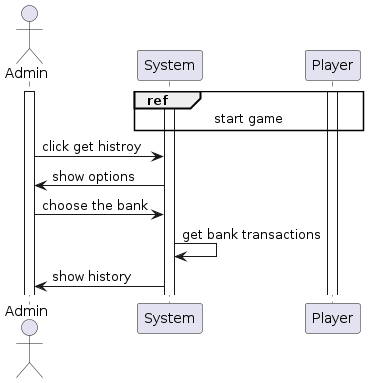
\includegraphics[height=3in]{../thesis_tex/assets/diagrams/see_transaction_history_of_bank_SD.png}
	 \caption{see transaction histroy of the bank by the admin actor Sequence Diagram}
\end{figure}

 \begin{figure}[H]
	 \centering
	 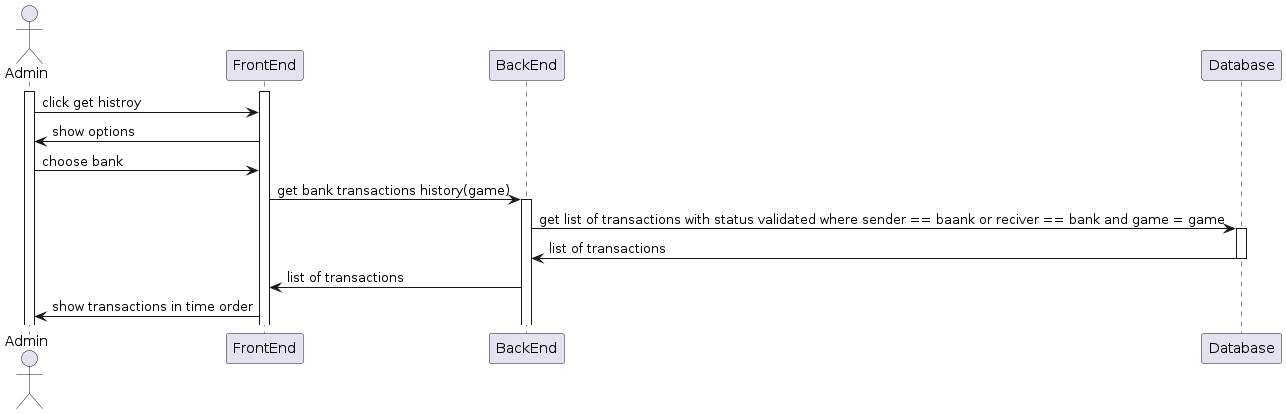
\includegraphics[height=4in,width=6in]{../thesis_tex/assets/diagrams/see_transaction_history_of_bank_detailedSD.png}
	 \caption{see transaction histroy of the bank by the admin actor detailed Sequence Diagram}
\end{figure}

\subsubsection{see transaction histroy of one player by the admin actor usecase}
 \begin{figure}[H]
	 \centering
	 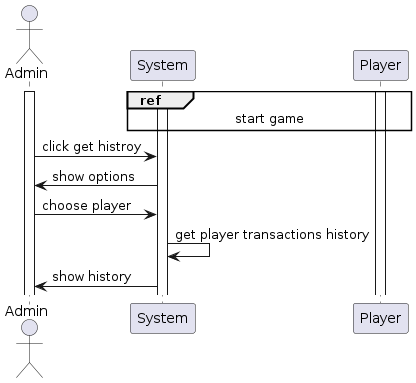
\includegraphics[height=3in]{../thesis_tex/assets/diagrams/see_transaction_history_of_one_player_SD.png}
	 \caption{see transaction histroy of one player by the admin actor Sequence Diagram}
\end{figure}

 \begin{figure}[H]
	 \centering
	 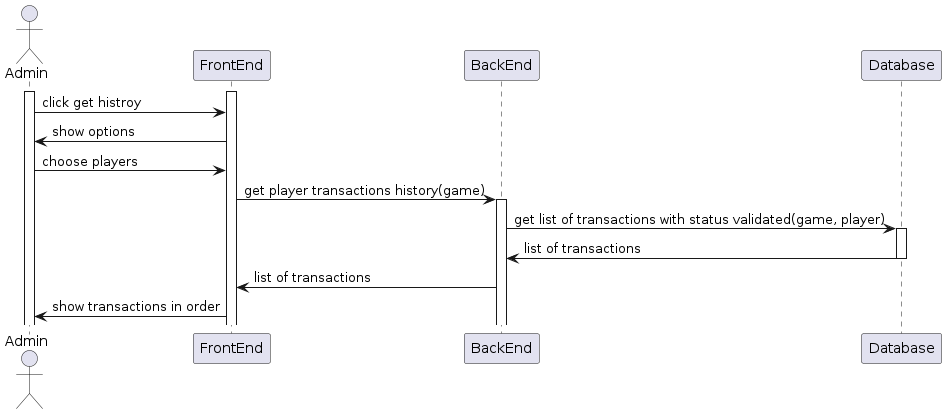
\includegraphics[height=4in,width=6in]{../thesis_tex/assets/diagrams/see_transaction_history_of_one_player_detailedSD.png}
	 \caption{see transaction histroy of one player by the admin actor detailed Sequence Diagram}
\end{figure}

\end{document}
